%
%  TODO:
%  - RELIRE POUR LES FOTTES ET ACCENTS accents faits, fottes a peu préfet
%  - le Q learning
%  -
%

\documentclass{report}
\usepackage{fontspec}
\usepackage{polyglossia}
\usepackage{pgfplots}
\usepackage{tikz}
\usepackage{unicode-math}
\usepackage{amsmath}
\usepackage{listings}
\usepackage{algorithm}
\usepackage{algpseudocode}
\usepackage{subfig}
\usepackage{hyperref}

\usetikzlibrary{patterns,arrows,positioning}

\setmainlanguage{french}

\newcommand{\R}{\mathbb{R}}

\DeclareMathOperator{\card}{card}
\DeclareMathOperator{\argmax}{argmax}
\DeclareMathOperator{\uniform}{Uniform}

\title{Ocaml---IA\\Tetris par Qlearning}
\author{C.~Cousin, G.~Hondet, L.~Pineau, B.~Viry}
\date{\today}

\tikzset{
    %Define standard arrow tip
    >=stealth',
    %Define style for boxes
    punkt/.style={
           rectangle,
           rounded corners,
           draw=black, very thick,
           text width=6.5em,
           minimum height=2em,
           text centered},
    % Define arrow style
    pildwn/.style={
           <-,
           thick,
           shorten <=2pt,
           shorten >=2pt,},
    pilup/.style={
           ->,
           thick,
           shorten <=2pt,
           shorten >=2pt,}
}


\begin{document}
\maketitle
\tableofcontents

\chapter*{Introduction}
\addcontentsline{toc}{chapter}{Introduction}

\chapter*{Notations}
\addcontentsline{toc}{chapter}{Notations}
Seront notées dans la suite du rapport:
\begin{itemize}
  \item \(n_t\) le nombre de tetrominos par jeu,
  \item \(\mathcal{S}\) l'ensemble des états,
  \item \(b_w, b_h\) la largeur et la hauteur totale du plateau.
\end{itemize}
Sauf mention explicite, les applications utiliseront les valeurs \(n_t=10000,
b_w = 6\). Seront distinguées la hauteur totale \(b_h\) et la hauteur relative
à un instant de jeu \(h\) du plateau, la première correspond à la hauteur
théorique maximale atteignable quand la deuxième concerne la hauteur
effectivement atteinte à un instant de jeu, i.e.\ le nombre de lignes non vides
sur le plateau.

\chapter{Tetris}

\section{Le jeu et sa simplification}
Tetris met le joueur au défi de réaliser des lignes complètes en déplaçant des
pièces de formes différentes, les tétrominos, qui défilent depuis le haut
jusqu'au bas de l'écran. Les lignes complétées disparaissent tout en rapportant
des points et le joueur peut de nouveau remplir les cases libérées. Le jeu
n'a pas de fin: le joueur perd la partie lorsqu'un tétromino reste bloqué en
haut.

Dans notre version simplifiée, il n'y a pas de limite de hauteur, le jeu se
termine après avoir fourni 10000 tetrominos à placer. De plus notre
tetris diffère par une grille plus étroite (6 colonnes disponibles), moins de
tetrominos différents (seulement 5) et des tetrominos plus petits (taille
inférieure à 2).

\begin{figure}[h]
  \centering
  \subfloat[Diagonale] {%
    
\begin{tikzpicture}
      \fill[color=magenta] (0,0) rectangle (1,1);
      \fill[color=magenta] (0,0) rectangle (-1,-1);
      \draw (-1,1) rectangle (1,-1);
    \end{tikzpicture}
  }\qquad
  \subfloat[L] {%
    
\begin{tikzpicture}
      \fill[color=cyan] (0,0) rectangle (1,1);
      \fill[color=cyan] (0,0) rectangle (-1,-1);
      \fill[color=cyan] (0,0) rectangle (-1,1);
      \draw (-1,1) rectangle (1,-1);
    \end{tikzpicture}
  }\qquad
  \subfloat[Carré] {%
    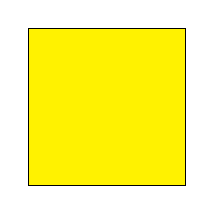
\begin{tikzpicture}
      \fill[color=yellow] (0,0) rectangle (1,1);
      \fill[color=yellow] (0,0) rectangle (-1,-1);
      \fill[color=yellow] (0,0) rectangle (-1,1);
      \fill[color=yellow] (0,0) rectangle (1,-1);
      \draw (-1,1) rectangle (1,-1);
    \end{tikzpicture}
  }\\
  \subfloat[Barre] {%
    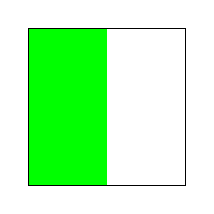
\begin{tikzpicture}
      \fill[color=green] (0,0) rectangle (-1,-1);
      \fill[color=green] (0,0) rectangle (-1,1);
      \draw (-1,1) rectangle (1,-1);
    \end{tikzpicture}
  }\qquad
  \subfloat[Point] {%
    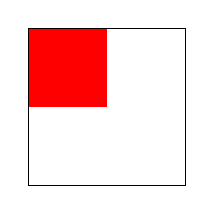
\begin{tikzpicture}
      \fill[color=red] (0,0) rectangle (-1,1);
      \draw (-1,1) rectangle (1,-1);
    \end{tikzpicture}
  }
  \caption{Liste des tertrominos}\label{fig:tetrolist}
\end{figure}

Un tetromino est placé par le choix d'une colonne et d'une orientation.

\section{L'implémentation}

\subsection{Représentation}

\paragraph{Tetrominos}
Les tetrominos sont tableaux de longueur 4. L'unidimensionnalité permet
d'implémenter les rotations comme des transformations d'indices, évitant la
création ou la modification de structures.

Les tetrominos sont tous de même dimension par souci d'homogénéité.

\paragraph{Plateau}
Le plateau est représenté par une matrice de dimension
\(2\cdot n_t \times 6\) d'entiers dans laquelle on inscrit les tetrominos. Les
manipulations du plateau se font en place.


\paragraph{Actions}
Composées d'une rotation et d'une translation. Elles permettent d'agir sur les
tetrominos. Les rotations sont représentées par les points cardinaux
(North, South, East, West) et les translations par un entier compris entre 0 et
\(b_w - 2\) correspondant à l'indice du coin supérieur gauche du tetromino
(voir fig\ref{fig:tetref}).

\begin{figure}[h]
  \centering
  \subfloat[Diagonale] {%
    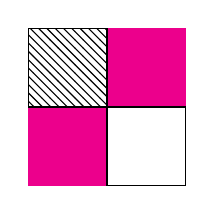
\begin{tikzpicture}
      \fill[color=magenta] (0,0) rectangle (1,1);
      \fill[color=magenta] (0,0) rectangle (-1,-1);
      \draw[pattern = north west lines] (0,0) rectangle (-1,1);
      \draw (0,0) rectangle (1,-1);
    \end{tikzpicture}
  }\qquad
  \subfloat[L] {%
    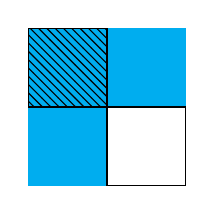
\begin{tikzpicture}
      \fill[color=cyan] (0,0) rectangle (1,1);
      \fill[color=cyan] (0,0) rectangle (-1,-1);
      \fill[color=cyan] (0,0) rectangle (-1,1);
      \draw[pattern = north west lines] (0,0) rectangle (-1,1);
      \draw (0,0) rectangle (1,-1);
    \end{tikzpicture}
  }
  \caption{Point de référence de tetromino, ici hachure}\label{fig:tetref}
\end{figure}

La géométrie de certains tetrominos rend certaines orientations redondantes. Par
exemple le carre est invariant par rotation, et utiliser les quatre rotations
ne fait qu'augmenter inutilement le nombre d'actions possibles, et augmente par
conséquent la quantité d'information que l'agent doit apprendre. Pour pallier
cette redondance, chaque tetromino dispose de son propre ensemble de rotations
applicables.

\section{Déroulement d'une partie}
Un tetromino choisi aléatoirement parmi les cinq disponibles est donne au
joueur. Ce dernier doit alors choisir ou et comment le placer. Une fois ce
choix effectue, le tetromino est place en respectant les contraintes du jeu. Le
plateau est ensuite mis a jour: les lignes complètes sont supprimées et la
hauteur est réévaluée. Un nouveau tetromino est donne et le jeu continue.


Lors d'une partie le joueur doit poser les pièces qui lui sont proposées sur
le plateau de jeu. Il est donc nécessaire d'utiliser une fonction \texttt{play}
qui permet de placer une pièce sur le plateau. La pièce ``tombe'' donc dans la
colonne sélectionnée tant qu'elle ne rencontre pas d'obstacle (fond du plateau
ou un autre tétromino). Pour cela, il y a besoin d'une fonction de test de
collision, qui renvoie si l'emplacement testé peut accueillir le tetromino.
S'il y a collision, on sélectionne le dernier emplacement libre et on place la
pièce.

Lorsqu'une ligne est entièrement remplie, elle est supprimée du tableau, mais
la taille totale du plateau reste la même.


\chapter{Q learning}

\section{Principe de l'apprentissage par renforcement et Q-learning}
\subsection{L'apprentissage par renforcement}

L'apprentissage par renforcement est une méthode d'apprentissage automatique
inspirée de la biologie. L'idée est un apprentissage à partir d'actions et
de récompenses, permettant \'a l'entité évoluant d'adapter son comportement aux
conséquences de ses actions.

Un agent est plongé dans un environnement (ici le jeu de Tetris) et effectue une
action (pour nous un mouvement). L'agent reçoit alors une récompense (ou alors
une punition) qui lui permet d'adapter son comportement et ainsi apprendre à
évoluer dans l'environnement.

\begin{figure}[h]
    \begin{center}
        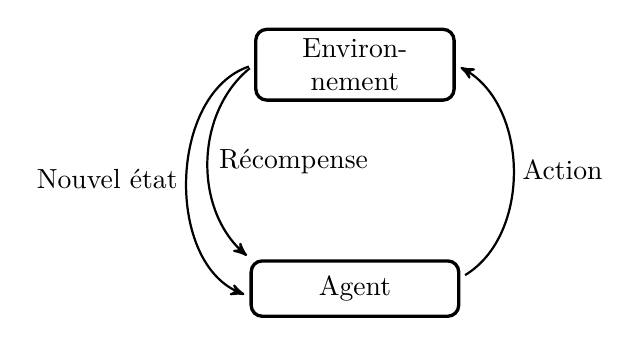
\begin{tikzpicture}[node distance=1cm, auto,]
         %nodes
         \node[punkt] (env) {Environnement};
         \node[punkt, inner sep=5pt,below=2cm of env]
         (agent) {Agent}
         edge[pilup,bend right=60] node[right] {Action} (env.east)
         edge[pildwn,bend left=70] node[left] {Nouvel état} (env.west)
         edge[pildwn,bend left=50] node[right] {Récompense} (env.west);
        \end{tikzpicture}
    \end{center}

    \caption{Principe d'apprentissage par renforcement}
    \label{}
\end{figure}

Le but de l'apprentissage va être de maximiser la somme des récompenses sur une
période donnée.

Plus formellement, notons:
\begin{itemize}
    \item \( s_i \) un état à l'étape \( i \)
    \item \( a_i \) une action jouée à l'étape \( i \)
    \item \( r(s_i, a_i) \) la récompense immédiate après l'action \( a_i \)
    \item \( \gamma \) la vision de l'agent (cf.~\ref{sec:algorithmes}).
\end{itemize}

La récompense à long terme pour un ensemble
\( s = (s_0, a_0, s_1, a_1, \hdots) \) est donc:
\[
  R(s) = \sum_{i=0}^{+\infty}\gamma^i \cdot r(s_i, a_i)
\]


\subsection{Le Q-learning}



\section{Représentation des états}

\subsection{Composition}
Intuitivement, un état correspond à la pièce donnée à jouer et la disposition
des pièces sur le plateau, ce qui correspond aux informations nécessaires pour
le placement d'une pièce par l'agent. En notant \(n_t\) le nombre de tetrominos
différents, \( h \) la hauteur du plateau a un instant considéré  et \(w\) la
largeur du plateau, on obtient \(n_t \cdot 2^{h \cdot b_w}\) états possibles.

Pour réduire le nombre d'états, on ne considère que les deux plus hautes lignes
contenant au moins un tetromino. On obtient \(5\cdot 2^{2 b_w}\) états
possibles, soit \(20480\) pour une largeur \( b_w = 6 \).

\subsection{Codage}
Comme chaque état correspond \textit{in fine} à une ligne de la matrice Q, il est
nécessaire d'avoir une bijection entre l'ensemble des états et les entiers. La
bijection génère deux représentations entières, une pour les deux lignes de
l'état et l'autre pour la pièce, et les combine en un état entier final,
\[
  \texttt{get\_state}\colon [0,4]\times [0, 2^{12} - 1] \to [0, 5\cdot 2^{12}].
\]


\section{Algorithmes}\label{sec:algorithmes}

L'algorithme~\ref{alg:action} concerne la manière dont l'agent choisit les
actions parmi l'ensemble des actions possibles \(\mathcal{A}\), étant donne un
état \(s\). Le paramètre \(\epsilon\) définit la fréquence de choix aléatoire.
\begin{algorithm}
  \caption{Choix de l'action}\label{alg:action}
  \begin{algorithmic}
    [1]
    \Procedure{ChooseAction}{$Q$, $s$, $\mathcal{A}$}
    \State{} tirage \(\gets \uniform([0, 1])\)
    \If{tirage \(> \epsilon\)}
    \Return{\(\argmax_{a\in\mathcal{A}} Q(s, a)\)}\Comment{Choix de l'action
    maximisant l'espérance de récompense}
    \Else{}
    \Return{\(\uniform(\mathcal{A})\)}\Comment{Choix aléatoire}
    \EndIf{}
    \EndProcedure{}
  \end{algorithmic}
\end{algorithm}


L'algorithme~\ref{alg:qlearning} définit la manière dont l'agent se met a jour
afin de maximiser l'espérance de gain. Est notée \(\gamma\) la vision de
l'agent correspondant a l'importance que l'agent attribue aux récompenses
futures par rapport a la récompense immédiate. Un \(\gamma\) de zéro crée un
agent myope ne choisissant son action que par rapport a la récompense immédiate
tandis qu'un \(\gamma\) tendant vers un associe autant d'importance aux
récompenses des coups suivants qu'a la récompense immédiate.
\begin{algorithm}
  \caption{Algorithme de \textit{Q-learning}}\label{alg:qlearning}
  \begin{algorithmic}
    [1]
    \Procedure{Update}{$Q$, $\epsilon$, $\gamma$, $\alpha$}
    \Repeat{}
    \State{} initialisation de \(s\)
    \Repeat{}
    \State{} \(a \gets\) ChooseAction$(Q, s, \mathcal{A}, \epsilon)$
    \State{} jouer \(a\), observer \(r\) et le nouvel \'etat \(s'\),
    \State{} \(Q(s, a) \gets Q(s, a) + \alpha\left[ r + \gamma \max_{a'}
      Q(s', a') - Q(s, a)\right]\)
    \Until{$s$ est terminal}
    \Until{entrainement fini}
    \EndProcedure{}
  \end{algorithmic}
\end{algorithm}

Pour réaliser une mise a jour, l'agent commence par choisir l'action qui, a un
état donne fournit l'espérance de récompense maximale, selon les connaissances
actuelles de l'agent. Une fois le coup joue, l'agent reçoit une récompense
évaluant évaluant l'impact du coup choisi sur l'environnement. L'agent utilise
cette récompense et sa connaissance des états résultants pour affiner
l'espérance de récompense associée au coup qu'il vient de réaliser.

\subsection{Paramètres}
L'apprentissage est paramétré par les trois variables,
\begin{itemize}
  \item \(\alpha \in [0, 1]\) le taux d'apprentissage,
  \item \(\epsilon \in [0, 1]\) la fréquence de coups aléatoires effectués,
  \item \(\gamma \in [0, 1]\) la vision de l'agent.
\end{itemize}
Pour assurer la convergence de la matrice vers la matrice optimale,
le taux d'apprentissage doit évoluer au cours des entrainements.
D'après~\cite{watkins92}, la suite \( (\alpha_k)_k \) doit vérifier
\( \sum_{k=0}^\infty \alpha_k = \infty \) et \(
\sum_{k=0}^\infty \alpha_k^2 \in \R \). La suite choisie a donc la forme
suivante, pour tout \( k \in \mathbb{N} \) et
\( C \in \R \backslash \{ \frac{-1}{k} \} \):
\[
  \alpha_k = \frac{1}{1 + Ck}.
\]
Le taux d'apprentissage reste manipulable via le paramètre \( C \).


% Le paramètre \(\epsilon\) pourra également varier au cours des jeux effectués.
% En effet, intuitivement, un \(\epsilon\) grand permet une exploration rapide de
% l'ensemble des états possibles mais devient nuisible lorsque la matrice est bien
% entrainée.

Le paramètre \(\epsilon\) répond au problème exploration contre exploitation. En
effet, un \(\epsilon\) important permet une exploration rapide de l'ensemble
des états possibles en jouant des actions aléatoires. À l'inverse un \(\epsilon\)
petit correspond à l'exploitation de la politique apprise par l'agent. Ainsi,
une diminution d'\(\epsilon\) au cours de la phase d'apprentissage permet de
stabiliser les résultats obtenus.

\begin{figure}
  \centering
  \subfloat[
    Premiers jeux, un \(\epsilon\) non nul favorise la prise de
    d\'ecisions pertinentes, visible sur les jeux 10 \`a 40 o\`u la courbe bleue
    (\(\epsilon = 0\)) est plus haute que les autres. De plus la courbe noire
    ayant le taux d'apprentissage le plus \'elev\'e est la plus basse.
  ] {%
    \begin{tikzpicture}
      \begin{axis}[line width=0.05, mark size = 0.1,
          legend entries={0,.0003,.0006,.0009}
        ]
        \foreach \i in {0,1,...,3}{%
          \addplot+ table [
            skip coords between index={100}{512},
            x expr = {\lineno}, y index = \i
          ] {data/epsilon.dat};
        }
      \end{axis}
    \end{tikzpicture}\label{sfig:exex_first_steps}
  }
  \quad
  \subfloat[
    Stabilisation, un \(\epsilon\) nul favorise l'utilisation des
    connaissances acquises et limite les mauvais jeux en \'evitant les actions
    inefficaces. La courbe ayant un taux d'apprentissage nul a une variance
    moindre.
  ] {%
    \begin{tikzpicture}
      \begin{axis}[line width=0.05, mark size = 0.1,
          legend entries={0,.0003,.0006,.0009}
        ]
        \foreach \i in {0,1,...,3}{%
          \addplot+ table [
            skip coords between index={0}{350},
            x expr = {\lineno}, y index = \i
          ] {data/epsilon.dat};
        }
      \end{axis}
    \end{tikzpicture}
  }
  \caption{Exploitation ou exploration?}
\end{figure}

\paragraph{Valeurs}
\begin{figure}
  \centering
  \begin{tikzpicture}
    \begin{axis}[line width=0.05, mark size = 0.1,
        legend entries={0.80,0.84,0.88,0.92,0.96,1.00}
      ]
      \foreach \i in {0,1,...,5}{%
        \addplot+ table [x expr = {\lineno}, y index = \i] {data/gamma.dat};
      }
    \end{axis}
  \end{tikzpicture}
  \caption{Influence du paramètre \(\gamma\)}
\end{figure}

\subparagraph{Taux d'apprentissage} Les courbes~\ref{sfig:exex_first_steps}
montrent qu'un \(\epsilon\) nul n'est pas optimal. Le
graphe~\ref{fig:learnrate_high} montre qu'un \(\epsilon\) plus grand que 0.02
tend a ralentir la convergence du système.



\chapter{Minimisation d'une fonction objectif \( V \)}

\section{Représentation des états et transitions}

Dans cette partie l'ensemble des états \( \mathcal{S} \) est égal à l'ensemble
des plateaux possibles. \( s \in \mathcal{S} \) est un plateau particulier.

\section{Nouvelle méthode d'apprentissage}

Pour s'affranchir de la limite de mémoire due au nombre d'états possibles, la
matrice est remplacée par une fonction objectif \( V \) tel que:
\[
  \forall s \in \mathcal{S}, \qquad V(s) =
  \mathbb{E}\left(\sum_{t=0}^{+\infty} \gamma ^t \cdot r_t\right)
\]
qui estime l'espérance de gain à partir d'un plateau donné.
L'apprentissage consiste donc maintenant à la maximisation de la
fonction \( V \).
On suppose \( V \) linéaire \(V \colon \R^n \to \R\). Cette fonction est alors
déterminée par un ensemble de poids \(w = (w_0\, w_1\, \dots\, w_n)^\top\)
qu'il va falloir ``entrainer''.

En notant \( s_t \) un plateau de jeu à un instant \( t \), et
\(\phi_i\colon \mathcal{S} \to \R\) des caractéristiques du plateau
(voir~\cite{boumaza13}), la fonction \(V\)
est définie par:
\[
  V \colon s_t \mapsto w_0 + \sum_{i=1}^n w_i \cdot \phi_i (s_t)
\]

On appelle transition un 4-uplet \( (s_t, a_t, r_t, s_{t+1}) \), Avec:
\begin{itemize}
    \item \( s_t \) le plateau à l'étape \( t \)
    \item \( a_t \) l'action joué à l'étape \( t \)
    \item \( r_t \) la récompense joué à l'étape \( t \)
    \item \( s_{t+1} \) le plateau résultant de l'action \( a_t \)
\end{itemize}


\section{Algorithme}

L'algorithme d'apprentissage utilisé dans cette partie repose sur une variante
stochastique de l'algorithme par descente de gradient.

L'idée est de jouer \( B \) coups et enregistrer dans une mémoire les différentes
transitions. Les coups sont choisis selon l'algorithme~\ref{alg:choseactionv2}.

\begin{algorithm}[h]
  \caption{Choix de l'action}\label{alg:choseactionv2}
  \begin{algorithmic}
    [1]
    \Procedure{ChooseAction2}{$V$, $s_t$, $\mathcal{A}$}
    \State{} tirage \(\gets \uniform([0, 1])\)
    \If{tirage \(> \epsilon\)}
    \State{}\Return{\(\argmax_{{a_t}\in\mathcal{A}} [r_t + \gamma V(s_{t+1})] \)}
    \\ \Comment{Choix de l'action maximisant l'espérance de récompense}
    \Else{}
    \State{}\Return{\(\uniform(\mathcal{A})\)}\Comment{Choix aléatoire}
    \EndIf{}
    \EndProcedure{}
  \end{algorithmic}
\end{algorithm}

Pour ne pas sauvegarder plusieurs fois le plateau de jeu \(s_t\), on ne met en
mémoire que les features intéressantes \( (\phi_1 (s_t), \hdots, \phi_7(s_t)) \).

Une fois la mémoire \( \mathcal{M} \) remplie avec \( B \) transitions, on
calcule \(\delta_t\):
\[
\forall t_t = (s_t, a_t, r_t, s_{t+1}) \in \mathcal{M},\quad
\delta(t_t) = \underbrace{r_t + \gamma \cdot V(s_{t+1})}_{target} -
\underbrace{V(s_{t})}_{prediction}
\]
Comme \( V \) estime l'espérance de gain, un agent bien entrainé doit annuler
les différents \(\delta_t\) (l'espérance prédite à l'instant t = la récompense
à l'instant t + l'espérance prédite à l'instant t + 1).

On définit alors une fonction de coût (loss function):
\[
\mathcal{L} = \frac{1}{2B} \sum _{t_t \in \mathcal{M}} \delta(t_t)^2
\]

On applique alors l'algorithme de descente de gradient pour minimiser la fonction
\( \mathcal{L} \) en actualisant les poids \( w \) suivant:
\[
w = w - \eta \nabla \mathcal{L}
\]

La procédure est synthétisé dans l'algorithme suivant:

\begin{algorithm}[H]
  \caption{Algorithme d'apprentissage d'une fonction linéaire}\label{alg:linfct}
  \begin{algorithmic}
    [1]
    \Procedure{Update}{$V$, $\epsilon$, $\gamma$, $\eta$, $\eta$}
    \Repeat{}
    \State{} initialisation de \(s\)
    \Repeat{}
    \For{1 to $B$}
    \State{} \(a \gets \mathup{ChooseAction2}(V, s, \mathcal{A}, \epsilon)\)
    \State{} joue \(a\), observer \(r\) et le nouvel \'etat \(s'\)
    \State{} ajouter a la mémoire \( \left(\phi(s), a, r, \phi(s')\right) \)
    \EndFor{}
    \State{} Choisir aléatoirement \(B\) quadruplets depuis la mémoire
    \State{} \(y_t \gets r_t + \gamma V\left(\phi(s_t')\right)\)
    \State{} \(\delta_t \gets y_t - V \left(\phi(s_t)\right)\)
    \State{} \(\mathcal{L} \gets \frac{1}{2B}\sum_{k=1}^B \delta_t^2\)
    \State{} \(w \gets w - \eta \nabla_w \mathcal{L}\)
    \Until{$s$ est terminal}
    \Until{Entrainement fini}
    \EndProcedure{}
  \end{algorithmic}
\end{algorithm}






\chapter{Programmes auxiliaires}
\section{Creation de faisceaux}\label{sec:faisceaux}
La création de faisceaux de courbes est automatisée via le script bash
\texttt{tetris\_parameval.bash}. Tout le paramétrage se fait en ligne de commande
par les arguments passés au script. Le langage bash a été choisi car semble le
plus propice a l'utilisation en ligne de commande.

Le parsing se fait avec le GNU \texttt{getopt}, les calculs en virgule flottante
avec \texttt{bc}. Les courbes sont ensuite produites via \texttt{gnuplot} et
les données sont enregistrées dans un fichier.



\section{Compilation}
La compilation du code source se fait via un \textit{makefile}. Il permet de
créer trois binaires,
\begin{itemize}
  \item le bytecode avec les options de debugging (\texttt{-g});
  \item le binaire optimisé pour bénéficier d'un temps d'exécution réduit;
  \item un toplevel avec tous les modules importés.
\end{itemize}

Les dépendances entre les modules sont gérées par \texttt{ocamldep}. La cible
\texttt{tags} permet de créer le fichier de tags utilisable par divers éditeurs.
La cible \texttt{doc} génère la documentation a l'aide de l'outil
\texttt{ocamldoc} et d'un code source documenté.




\section{Rapport}
Le rapport est rédigé en \LaTeX{}, les figures et graphes sont faits grâce a
\texttt{PGF/tikz}. Le rapport est compilé via un \textit{makefile} dédié
automatisant la génération des fichiers de données pour créer les courbes en
appelant le script bash susmentionne en~\ref{sec:faisceaux}. Le
programme \texttt{latexmk} est également utilisé pour faciliter la compilation.




\chapter{Difficultés rencontrées}

\section{Limites intrinsèques de conception}
\subsection{Résolution de collisions}
La gestion actuelle des collisions oblige l'accessibilité de la position finale
depuis le haut du plateau. L'agent ne peut placer de tetrominos qu'\'a des
positions o\'u ils peuvent ``tomber'', c'est-\'a-dire que les tetrominos ne
peuvent être glissés au dernier moment sous d'autres. Plus formellement, tout
tetromino placé ne peut avoir de cellule occupée en amont des siennes. Autrement
dit, en considérant un tetromino de largeur \(l\) (avec dans notre
implémentation \(l = 1\) ou \(2\)), chacun des tétraèdres composant le tetromino
ne peut avoir de tétraèdre d'un tetromino pose précédemment sur la même colonne
a une hauteur supérieure.

\section{Le fléau de la mutabilité}
L'usage du \texttt{Array.blit} s'est révélé plus délicat que prévu. En
considerant que la ligne \(l\) doit être supprimée et en notant \(h\) la hauteur
actuelle du plateau, le principe est de copier la section de tableau incluant
les lignes \(l+1\) jusqu'à \(h+1\) une ligne en dessous, i.e.\ translater le
bloc d'une ligne vers le bas.

Cette démarche engendre des comportements anormaux car la ligne \(h+1\) n'est
pas copiée sur la ligne \(h\), elles partagent la même adresse mémoire. Ainsi,
il était observé quelques coups après un blit un dédoublement de carrés de
tetrominos, faisant augmenter la hauteur.

Pour pallier ce problème de partage d'adresse mémoire, la ligne \(h\) est
recréée à chaque blit.

\section{Hollandais volant}\label{sec:hollandais_volant}
La fonction collide permet de tester la collision du tetromino avec les autres
pièces et le fond du plateau. Lors de l'exécution de la fonction \texttt{play}
on testait donc toutes les positions possibles pour déposer les pièces de
dimension 2 \(\times \) 2 sur le fond du plateau s'il n'y avait pas eu de
collision. Malheureusement, certaines pièces comme le point ou la ligne
pouvaient avoir une ``ligne vide'' en bas sous certaines rotations. Pour
résoudre ce problème qui est devenu évident après la résolution du problème de
\texttt{Array.blit}, nous avons décidé de restreindre les états possibles dans
la Q-matrice. En effet lors de l'initialisation de la Q-matrice, tous les états
accessibles sont mis à 0 (flottant) et tous les états non utilisés sont
initialisés à \(-\infty \). Ainsi, pour le point, on ne gardera que les
rotations \texttt{South} et \texttt{West}.

\section{Le foncteur n'est pas passé}
Ayant deux moyens pour résoudre le tetris, il semble pertinent de
généraliser le code afin de faire en sorte que toute implémentation
d'agent soit facilement développable et intégrable au reste du projet. Pour
cela un foncteur semble pertinent: le foncteur \texttt{Agent.Make} prendrait en
paramètre un module d'implémentation d'agent, contenant une fonction
permettant de choisir une action, un fonction de mise \`a jour de l'agent, un
type d\'esignant la donnée avec laquelle travaille l'agent (e.g.\ matrice de
flottants pour le Q learning et tableau de poids flottants pour la fonction de
valuation). Le r\'esultat de l'application de ce foncteur est un module ayant
une fonction \texttt{train} entra\^inant en place l'agent, une fonction
\texttt{play} pour jouer un jeu de tetris et une fonction make pour cr\'eer un
agent initial.

La généralisation du code s'est malheureusement révélée plus
délicate que prévu. D'une part les deux méthodes implémentées
différaient trop, notamment sur le nombre de paramètres, ou
l'utilisation d'une mémoire, d'autre part adapter le code \'a ces deux
implémentations finissait plus \'a ressembler \'a du bricolage plutôt qu'\'a
de la généralisation. Et de plus cela avait tendance \'a pervertir le code
développé pour la fonction de valuation, le poussant \'a coller \'a la
signature d'un argument de foncteur qui est peut-être, avouons le, mal conçu.

En conséquence, l'agent utilisant la fonction d'évaluation est codé sur
une branche dédiée du git, la branche \texttt{valuation}. Le code du
foncteur est disponible sur la branche \texttt{functorise}.
\chapter{Résultats du projet}

\chapter*{Conclusion}
\addcontentsline{toc}{chapter}{Conclusion}

\begin{thebibliography}{9}
    \bibitem{watkins92}
    Christopher~J.C.H.~Watkins, Peter~Dayan,
    \textit{Q-Learning, Machine Learning}
    1992.
    \bibitem{deepmind}
    Voloddymyr~Mnih, Koray Kavukcuoghlu, David Silver, Alex Graves, Ioannis
    Antonoglou, Daan Wierstra, Martin Riedmiller,
    \textit{Playing Atari with Deep Reinforcement Learning}
    \bibitem{boumaza13}
    Amine Boumaza,
    \textit{How to design good Tetris players}
    2013.
\end{thebibliography}

\end{document}
